In the previous sections we described ROMC from the user's
point-of-view; the demonstration focused on performing the inference
with the ready-to-use tools. Apart from this use-case, a practitioner
can also use the implementation as a meta-algorithm, adding custom
algorithms as part of the method. Our implementation allows such
intervention. In the rest of the chapter, We will initially present
the main internal classes and then we will exhibit how to add custom
methods.

\subsubsection{Entities presentation}

In figure \ref{fig:example_training} we provide an overview of the
classes used. The class $\pinline{ROMC}$ can be thought as the
interface between the user and the method. The rest of the classes are
responsible for the backend functionality. It is important for the
reader to understand the sequence of the events for performing the
inference, as demonstrated in figure \ref{fig:romc_overview}.

The initialisation of the ROMC object sets the attributes
\pinline{model, model_prior, bounds, inference_state}; the rest of the
attributes are set to \pinline{None}.\footnote{in all cases, we use
  the value None for indicating that an attribute is not yet
  initialised."} The \pinline{_sample_nuisance()} routine samples
$n_1$ integers for the discrete integer uniform distribution. The
\pinline{_define_objectives()} routine initialises $n_1$
\pinline{OptimisationProblem} objects, appends them to a
\pinline{List} and sets the \pinline{List} to the
\pinline{romc.optim_problems} attribute. The
\pinline{OptimisationProblem} objects have the attributes
\pinline{objective, bounds} defined; all the rest are set to
\pinline{None}. The objective attribute, which is a
\pinline{Callable}, is created by setting the seed of the
\pinline{model.generate()} function to the corresponding integer,
turning the random generator to a deterministic. Afterwards, depending
on the boolean argument \pinline{use_bo=True/False}, the
\pinline{_solve_gradients} or the \pinline{_solve_bo} routine is
called. Both of them, for each optimisation problem, they solve it and
initialise a \pinline{RomcOptimisationResult} object and store it to
the \pinline{OptimisationProblem.result} attribute. However, each
method applies a different optimisation scheme using different methods
under the hood; \pinline{_solve_gradients} calls the
\pinline{minimize} class of the \pinline{scipy.optimize} library
\autocite{2020SciPy-NMeth}, whereas \pinline{_solve_bo} initialises a
\pinline{BoDeterministic} object for performing the
optimisation.\pinline{BoDeterministic} is a class we implemented for
performing Bayesian Optimisation and fitting a Gaussian Process
surrogate model to the objective function. In turn, the
\pinline{BoDeterministic} class relies on the Gpy framework
\autocite{gpy2014} for fitting the Gaussian Process. The only
difference between \pinline{_solve_gradients} and \pinline{_solve_bo},
at the software level, is the initialisation of the
\pinline{OptimisationProblem.surrogate} attribute with a
\pinline{Callable} that wraps the \pinline{GPyRegression.predict_mean}
function. If \pinline{_solve_gradients} is called, remains
\pinline{None}. Afterwards, \pinline{_filter_solutions} is called with
an argument \pinline{eps_region} to discard the optimal distances that
are over the threshold. Afterwards, \pinline{_build_boxes} estimates
the bounding boxes around the accepted objective functions. For each
accepted objective function, a \pinline{RegionConstructor} is
initialised to construct the region(s). In the current implementation,
for each objective function we constract a single bounding box, but
this may not be the case in a future approach; for being able to
support multiple bounding boxes per objective function, we decided to
return a \pinline{List} of \pinline{NDimBoundingBox}
objects\footnote{Each \pinline{NDimBoundingBox} object represents a
  region.} The \pinline{List} initialises the
\pinline{OptimisationProblem.regions} attribute. After that, if the
\pinline{fit_models} arguments is \pinline{True}, the
\pinline{_fit_models} routine is called before
\pinline{_define_posterior}\footnote{Otherwise, the
  \pinline{_define_posterior} is called immediately.}. The routine
\pinline{_fit_models}, for each objective function, fits a quadratic
model on the area around the optimal point. For doing so, it creates a
small training set by getting samples from \pinline{NDimBoundingBox}
and evaluating the objective function at those points. Afterwards,
based on these points, it fits a quadratic model using the
\pinline{linear_model.LinearRegression} and
\pinline{preprocessing.PolynomialFeatures} functions of the
\pinline{scikit-learn} package \autocite{scikit-learn}. Finally, the
\pinline{_define_posterior} collects the bounding boxes
(\pinline{OptimisationProblem.regions}) and the objective functions
(\pinline{OptimisationProblem.objective} and
\pinline{OptimisationProblem.surrogate} and
\pinline{OptimisationProblem.local_surrogate}) to initialise a
\pinline{RomcPosterior} object. The \pinline{RomcPosterior} objects
initialise the \pinline{ROMC.posterior} attribute.


\begin{figure}[h]
    \begin{center}
      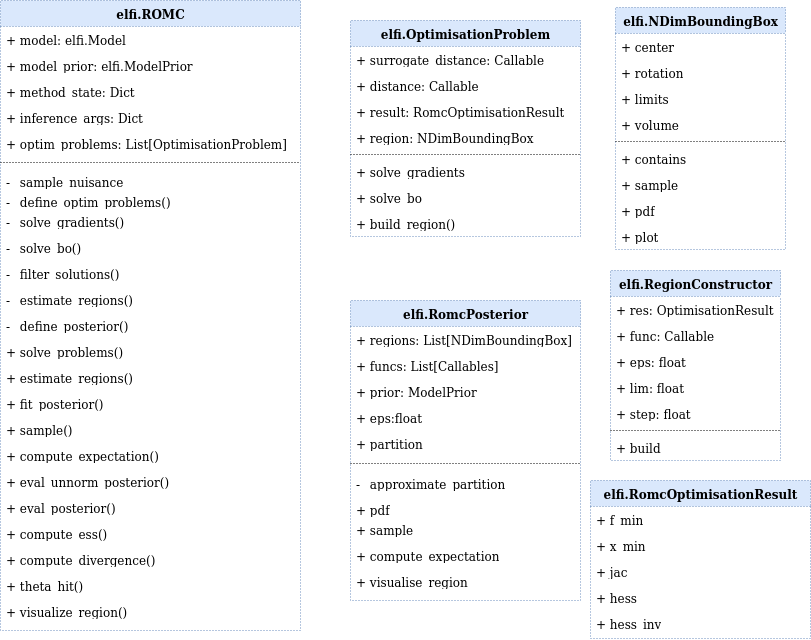
\includegraphics[width=\textwidth]{./Thesis/graphs/RomcEntityDiagram.png}
    \end{center}
  \caption{Histogram of distances and visualisation of a specific region.}
  \label{fig:example_training}
\end{figure}


\subsubsection{Extensibility of the ROMC method}

In this section we will explain how a researcher may replace some
parts of the ROMC method with his/her custom alogorithms easily.

Treating the ROMC inference approach as a meta-algorithm, we can
locate at least four replacable parts, where a researcher may
experiment with novel algorithms, keeping the rest of the method
unchanged. These are (a) solving the problems with a gradient based
method (b) solving the problems without gradients (Bayesian
Optimisation is not the unique single approach) (c) constructing the
bounding boxes and (d) fitting local surrogate models. Each of the
aforementioned tasks may be approached with fundamentally different
algorithms than the ones we propose without the rest of the method to
change. We take care so that a researcher may replace the specific
parts, without too much work, by isolating in our designing the
entities that operate in those parts from the rest of the code.

It is important to clarify that the basic class \pinline{ROMC} which
is used as an interface between the user and the backend should not be
altered at all; tha \pinline{ROMC} class represents the steps that
ROMC should perform as a meta-algorithm, without being influenced by
the "back-end" functionalities that perform these steps. For having
this ..., the routines that call those backend functionalities define
a dynamic dictionary arguments, where the user may pass all
keyword-arguments that are needed e.g.\
\pinline{_solve_gradients(**kwargs)}, \pinline{_solve_bo(**kwargs)},
\pinline{_build_boxes(**kwargs)},
\pinline{_fit_models(**kwargs)}. These mathods do nothing more than
accesing all \pinline{OptimisationProblem} one after the other and
call the corresponding function
i.e.\pinline{solve_gradients(**kwargs)}, \pinline{solve_bo(**kwargs)},
\pinline{build_region(**kwargs)},
\pinline{fit_local_surrogate(**kwargs)}. The functions of
\pinline{OptimisationProblem} execute their main functionality and
update the appropriate attribute. Table \ref{tab:extensibility}
summarizes this procedure.

\begin{center} \label{tab:extensibility}
\captionof{table}{Table explaining the object returned by each
  \pinline{OptimisationProblem} routine. The functions of the first
  column (\pinline{ROMC} class) call the correpsonding functions of
  the second column (\pinline{OptimisationProblem} class). The
  functions of the second column should execute their main
  functionality and update the appropriate attribute with a certain
  object, as described in the third column. }
  
\begin{tabular}{ c|c|c }
\hline
\pinline{ROMC} & \pinline{OptimisationProblem} & \pinline{Return value} \\
\hline \hline
\pinline{_solve_gradients()} & \pinline{solve_gradients()} & \pinline{result <- RomcOptimisationResult} \\
\hline
  \multirow{ 2}{*}{\pinline{_solve_bo()}} & \multirow{ 2}{*}{\pinline{solve_bo()}} & \pinline{result <- RomcOptimisationResult} \\
  & & \pinline{surrogate <- Callable} \\
\hline
\pinline{_build_boxes()} & \pinline{build_region()} & \pinline{regions <- List[NDimBoundingBox]}\\
\hline
  \pinline{_fit_models()} & \pinline{fit_local_surrogate()} & \pinline{local_surrogate <- Callable}\\
  \hline
\end{tabular}
\end{center}

\subsubsection*{Example: use a Neural Network as a local surrogate model}

Let's say we have observed that the local area around $\theta_i^*$ is
too complex to be represented by a simple quadratic model, as in the
current implementation. Hence, a researcher thinks of using a more
agile model and selects a neural network as a good alternative. In the
following snippet, we demonstrate how he could implement this
functionality, without much effort; (a) he has to develop the neural
network using the package of his choice (b) he must create a custom
optimisation class, inheriting the basic \pinline{OptimisationClass}
and (c) he has to overwrite the \pinline{fit_local_surrogate} routine,
with one that sets the neural network's prediction function as the
\pinline{local_surrograte} attribute. The argument \pinline{**kwargs}
may be used for passing all the important arguments e.g.\ training
epochs, gradient step etc. If he would like to set the size of the
training set dynamically, we may replace \pinline{x =
  self.regions[0].sample(30)} with \pinline{x =
  self.regions[0].sample(kwargs["nof_examples"])}.

\begin{pythoncode}
  class NeuralNetwork:
      def __init__(self, **kwargs):
          # set the input arguments

      def train(x, y):
          # training code

      def predict(x):
          # prediction code

  # Inherit the base optimisation class
  class customOptim(elfi.methods.parameter_inference.OptimisationProblem):
      def __init__(self, **kwargs):
          super(customOptim, self).__init__(**kwargs)

      # overwrite the function you want to replace
      def fit_local_surrogate(**kwargs):
          # init and train the NN
          x = self.regions[0].sample(30) # 30 training points
          y = [np.array([self.objective(ii) for ii in x])]
          nn = NeuralNet()
          nn.train(x,y)

          # set the appropriate attribute
          self.local_surrogate = nn.predict

          # update the state
          self.state["local_surrogate"] = True

  # pass the custom inference method as argument
  romc = elfi.ROMC(dist, bounds, custom_optim_class=customOptim)
\end{pythoncode}


The above method, for 